%%%%%%%%%%%%%%%%%%%%%%%%%%%%%%%%%%%%%%%%%%%%%%%%%%%%%%%%%%%%%%%%%%%%%%%%%%%%
% AGUJournalTemplate.tex: this template file is for articles formatted with LaTeX
%
% This file includes commands and instructions
% given in the order necessary to produce a final output that will
% satisfy AGU requirements, including customized APA reference formatting.
%
% You may copy this file and give it your
% article name, and enter your text.
%
% guidelines and troubleshooting are here: 

%% To submit your paper:
\documentclass[draft]{agujournal2019}
\usepackage{url} %this package should fix any errors with URLs in refs.
\usepackage{lineno}
\usepackage[inline]{trackchanges} %for better track changes. finalnew option will compile document with changes incorporated.
\usepackage{soul}
\usepackage{wrapfig}
\linenumbers
%%%%%%%
% As of 2018 we recommend use of the TrackChanges package to mark revisions.
% The trackchanges package adds five new LaTeX commands:
%
%  \note[editor]{The note}
%  \annote[editor]{Text to annotate}{The note}
%  \add[editor]{Text to add}
%  \remove[editor]{Text to remove}
%  \change[editor]{Text to remove}{Text to add}
%
% complete documentation is here: http://trackchanges.sourceforge.net/
%%%%%%%

\draftfalse

%% Enter journal name below.
%% Choose from this list of Journals:
%
% JGR: Atmospheres
% JGR: Biogeosciences
% JGR: Earth Surface
% JGR: Oceans
% JGR: Planets
% JGR: Solid Earth
% JGR: Space Physics
% Global Biogeochemical Cycles
% Geophysical Research Letters
% Paleoceanography and Paleoclimatology
% Radio Science
% Reviews of Geophysics
% Tectonics
% Space Weather
% Water Resources Research
% Geochemistry, Geophysics, Geosystems
% Journal of Advances in Modeling Earth Systems (JAMES)
% Earth's Future
% Earth and Space Science
% Geohealth
%
% ie, \journalname{Water Resources Research}

\journalname{Enter journal name here}


\begin{document}

%%%%%%%%%%%%%%%%%%%%%%%%%%%%%%%%%%%%%%%%%%%%%%%
%  TITLE
%
% (A title should be specific, informative, and brief. Use
% abbreviations only if they are defined in the abstract. Titles that
% start with general keywords then specific terms are optimized in
% searches)
%
%%%%%%%%%%%%%%%%%%%%%%%%%%%%%%%%%%%%%%%%%%%%%%%

% Example: \title{This is a test title}

\title{=enter title here=}

%%%%%%%%%%%%%%%%%%%%%%%%%%%%%%%%%%%%%%%%%%%%%%%
%
%  AUTHORS AND AFFILIATIONS
%
%%%%%%%%%%%%%%%%%%%%%%%%%%%%%%%%%%%%%%%%%%%%%%%

% Authors are individuals who have significantly contributed to the
% research and preparation of the article. Group authors are allowed, if
% each author in the group is separately identified in an appendix.)

% List authors by first name or initial followed by last name and
% separated by commas. Use \affil{} to number affiliations, and
% \thanks{} for author notes.
% Additional author notes should be indicated with \thanks{} (for
% example, for current addresses).

% Example: \authors{A. B. Author\affil{1}\thanks{Current address, Antartica}, B. C. Author\affil{2,3}, and D. E.
% Author\affil{3,4}\thanks{Also funded by Monsanto.}}

\authors{=list all authors here=}


% \affiliation{1}{First Affiliation}
% \affiliation{2}{Second Affiliation}
% \affiliation{3}{Third Affiliation}
% \affiliation{4}{Fourth Affiliation}

\affiliation{=number=}{=Affiliation Address=}
%(repeat as many times as is necessary)


% Corresponding author mailing address and e-mail address:

% (include name and email addresses of the corresponding author.  More
% than one corresponding author is allowed in this LaTeX file and for
% publication; but only one corresponding author is allowed in our
% editorial system.)

% Example: \correspondingauthor{First and Last Name}{email@address.edu}

\correspondingauthor{=name=}{=email address=}



%%%%%%%%%%%%%%%%%%%%%%%%%%%%%%%%%%%%%%%%%%%%%%%
% KEY POINTS
%%%%%%%%%%%%%%%%%%%%%%%%%%%%%%%%%%%%%%%%%%%%%%%
%  List up to three key points (at least one is required)
%  Key Points summarize the main points and conclusions of the article
%  Each must be 140 characters or fewer with no special characters or punctuation and must be complete sentences

% Example:
% \begin{keypoints}
% \item	List up to three key points (at least one is required)
% \item	Key Points summarize the main points and conclusions of the article
% \item	Each must be 140 characters or fewer with no special characters or punctuation and must be complete sentences
% \end{keypoints}

\begin{keypoints}
\item enter point 1 here
\item enter point 2 here
\item enter point 3 here
\end{keypoints}

%%%%%%%%%%%%%%%%%%%%%%%%%%%%%%%%%%%%%%%%%%%%%%%
%
%  ABSTRACT and PLAIN LANGUAGE SUMMARY
%
% A good Abstract will begin with a short description of the problem
% being addressed, briefly describe the new data or analyses, then
% briefly states the main conclusion(s) and how they are supported and
% uncertainties.

% The Plain Language Summary should be written for a broad audience,
% including journalists and the science-interested public, that will not have 
% a background in your field.
%
% A Plain Language Summary is required in GRL, JGR: Planets, JGR: Biogeosciences,
% JGR: Oceans, G-Cubed, Reviews of Geophysics, and JAMES.
% see http://sharingscience.agu.org/creating-plain-language-summary/)
%
%%%%%%%%%%%%%%%%%%%%%%%%%%%%%%%%%%%%%%%%%%%%%%%

%% \begin{abstract} starts the second page

\begin{abstract}
[ enter your Abstract here ]
\end{abstract}

\section*{Plain Language Summary}
Enter your Plain Language Summary here or delete this section.
Here are instructions on writing a Plain Language Summary: 
https://www.agu.org/Share-and-Advocate/Share/Community/Plain-language-summary


%%%%%%%%%%%%%%%%%%%%%%%%%%%%%%%%%%%%%%%%%%%%%%%
%
%  BODY TEXT
%
%%%%%%%%%%%%%%%%%%%%%%%%%%%%%%%%%%%%%%%%%%%%%%%

%%% Suggested section heads:
% \section{Introduction}
%
% The main text should start with an introduction. Except for short
% manuscripts (such as comments and replies), the text should be divided
% into sections, each with its own heading.

% Headings should be sentence fragments and do not begin with a
% lowercase letter or number. Examples of good headings are:

% \section{Materials and Methods}
% Here is text on Materials and Methods.
%
% \subsection{A descriptive heading about methods}
% More about Methods.
%
% \section{Data} (Or section title might be a descriptive heading about data)
%
% \section{Results} (Or section title might be a descriptive heading about the
% results)
%
% \section{Conclusions}

\section{Introduction}\label{intro}
% examples of citation formatting: 
% \cite{Arthun2012}
% \citeA{Arthun2012}

% global context, why are we interested in the Arctic, Arctic Amplification; regional feedback mechanisms with sea ice loss, how does Arctic circulation, heat fluxes and water masses require use to understand transformation process
% FIGURE 1 to include: an Arctic map of Bathymetry or two of heat/freshwater content anomalies
% mean velocity of the Barents Sea AW layer to show the direction of flow
% history of amplification
The Arctic has undergone substantial climatic shifts in recent decades, with air temperatures rising more rapidly than anywhere else on Earth \cite{Cosimo2014,Carmack2015}. This accelerated warming has led to significant declines in sea ice extent and thickness \cite{Perovich2009,Onarheim2018,Stroeve2018}, with the most pronounced changes in the Barents Sea \cite{Onarheim2017}. The increase in surface air temperature (SAT), a phenomenon known as Arctic Amplification \cite{Manabe1980}, is correlated with these reductions in sea ice and a notable warming signal in the upper ocean \cite{Serreze2009,Screen2010,Pithan2014,Marshall2014}. These changes can alter Barents Sea mixed layer salinity \cite{Lind2018} and net primary production, changing migratory patterns of fish and marine mammals and signaling a regime shift in a process known as borealization \cite{Fossheim2015,Polyakov2020_borealization,Ingvaldsen2021}. Moreover, Arctic warming in the lower troposphere may impact midlatitude weather \cite{Honda2009,Petoukhov2010,Cohen2014}. Several positive feedback mechanisms, including lapse rate, surface albedo reduction, and increased atmospheric water vapor, are thought to reinforce observed warming \cite{Pithan2014,Timmermans2018,Pistone2019,Previdi2021}. However, Arctic Amplification is nonuniform and intensified in the Northern Barents Sea \cite{Previdi2021,Rantanen2022}, yet some models still underestimate observed trends \cite{Huang2017}. In light of these changes, a deeper understanding of the drivers of ocean heat and salt content variability is urgently needed.

% the Barents Sea as a gateway to the Arctic/Atlantification; how does AW inflow influence Barents Sea thermohaline circulation and regional transformations; role of Barents Sea in regulating heat and freshwater exchange, why does this merit investigation regionally
These amplified changes are particularly evident in the Barents Sea, which acts as a transition zone between the Atlantic and Arctic Oceans. The Barents Sea plays a critical role in regulating heat and freshwater exchange between these two basins and serves as a conduit for Atlantic Water (AW), the primary heat source for the Arctic \cite{Smedsrud2013} and am important driver of Arctic Ocean warming \cite{Oldenburg2024}. The region is characterized by two distinct regimes: the southern part dominated by Atlantic Water (AW) inflow \cite{Hakkinen2009}, and the northern having seasonal sea ice coverage and more Arctic conditions. In the northern regime, salinity-driven stratification mirrors that of the central Arctic \cite{Nansen1902,Carmack2007}, with a surface mixed layer, a near-surface cold and fresh Arctic Water layer, and an underlying warm and salty Atlantic layer \cite{Loeng1991,Rudels2022} kept at depth by freshwater input from ice melt \cite{Lind2016,Lundesgaard2022}. However, recent studies have highlighted the relationship between amplified hotspot in the North with increasing heat advected through the Barents Sea Opening (BSO), contributing to sea ice retreat \cite{Arthun2012,Li2017} as well as weaker stratification and enhanced vertical mixing and upward heat transfer \cite{Lind2018,Gerland2023}, limiting sea ice formation \cite{Barton18,Wang2019}. This phenomenon is referred to as "Atlantification", has resulted in a northward expansion of the more Atlantic regime of the Barents Sea, with implications for the local ecology \cite{Bogstad2015,Dalpadado2014,Ingvaldsen2021}. Furthermore, because the heat carried by AW is enough to melt the sea ice of the internal Arctic were it to reach the surface, the Atlantification of the Barents Sea has resulted in warmed outflows, with implications for Arctic-wide transformations \cite{Polyakov2017,Skagseth2020,Grabon2021}. As the Barents Sea becomes a more Atlantic-dominated regime, its capacity for cooling is declining, with consequences for the heat carried to the Arctic \cite{Smedsrud2022}. Thus, it is essential to understand how surface forcing, Atlantic inflow, and internal mixing jointly contribute to heat and freshwater variability, shaping both regional and Arctic-wide transformations.

%%%%%%%%%%%%%%%%%%%%%

% physical changes in the Barents Sea: observed trends, recent studies, sea ice extent and seasonal variability, focus on how reduced sea ice interacts with advective inflow; ongoing WMT including conversion of AW to Arctic Water through heat loss with transport through Barents Sea
% FIGURE 2: the two regimes identified in map view, a comparison of theta change with depth
% timeseries of sea ice extent, freshwater content of Barents Sea, theta with depth
(DRAFT) The upper ocean heat content of of the Barents sea increased steadily from 2003--2017 (Fig~\ref{fig:timeseries}). The upper ocean freshwater content decreased by 50\% during the first five years of this period, remained steady until 2013, then increased from 2013--2017. At the same time, sea ice extent has been steadily declining throughout this period, with minima in 2012 and 2016.

\begin{wrapfigure}{r}{0.5\textwidth}
    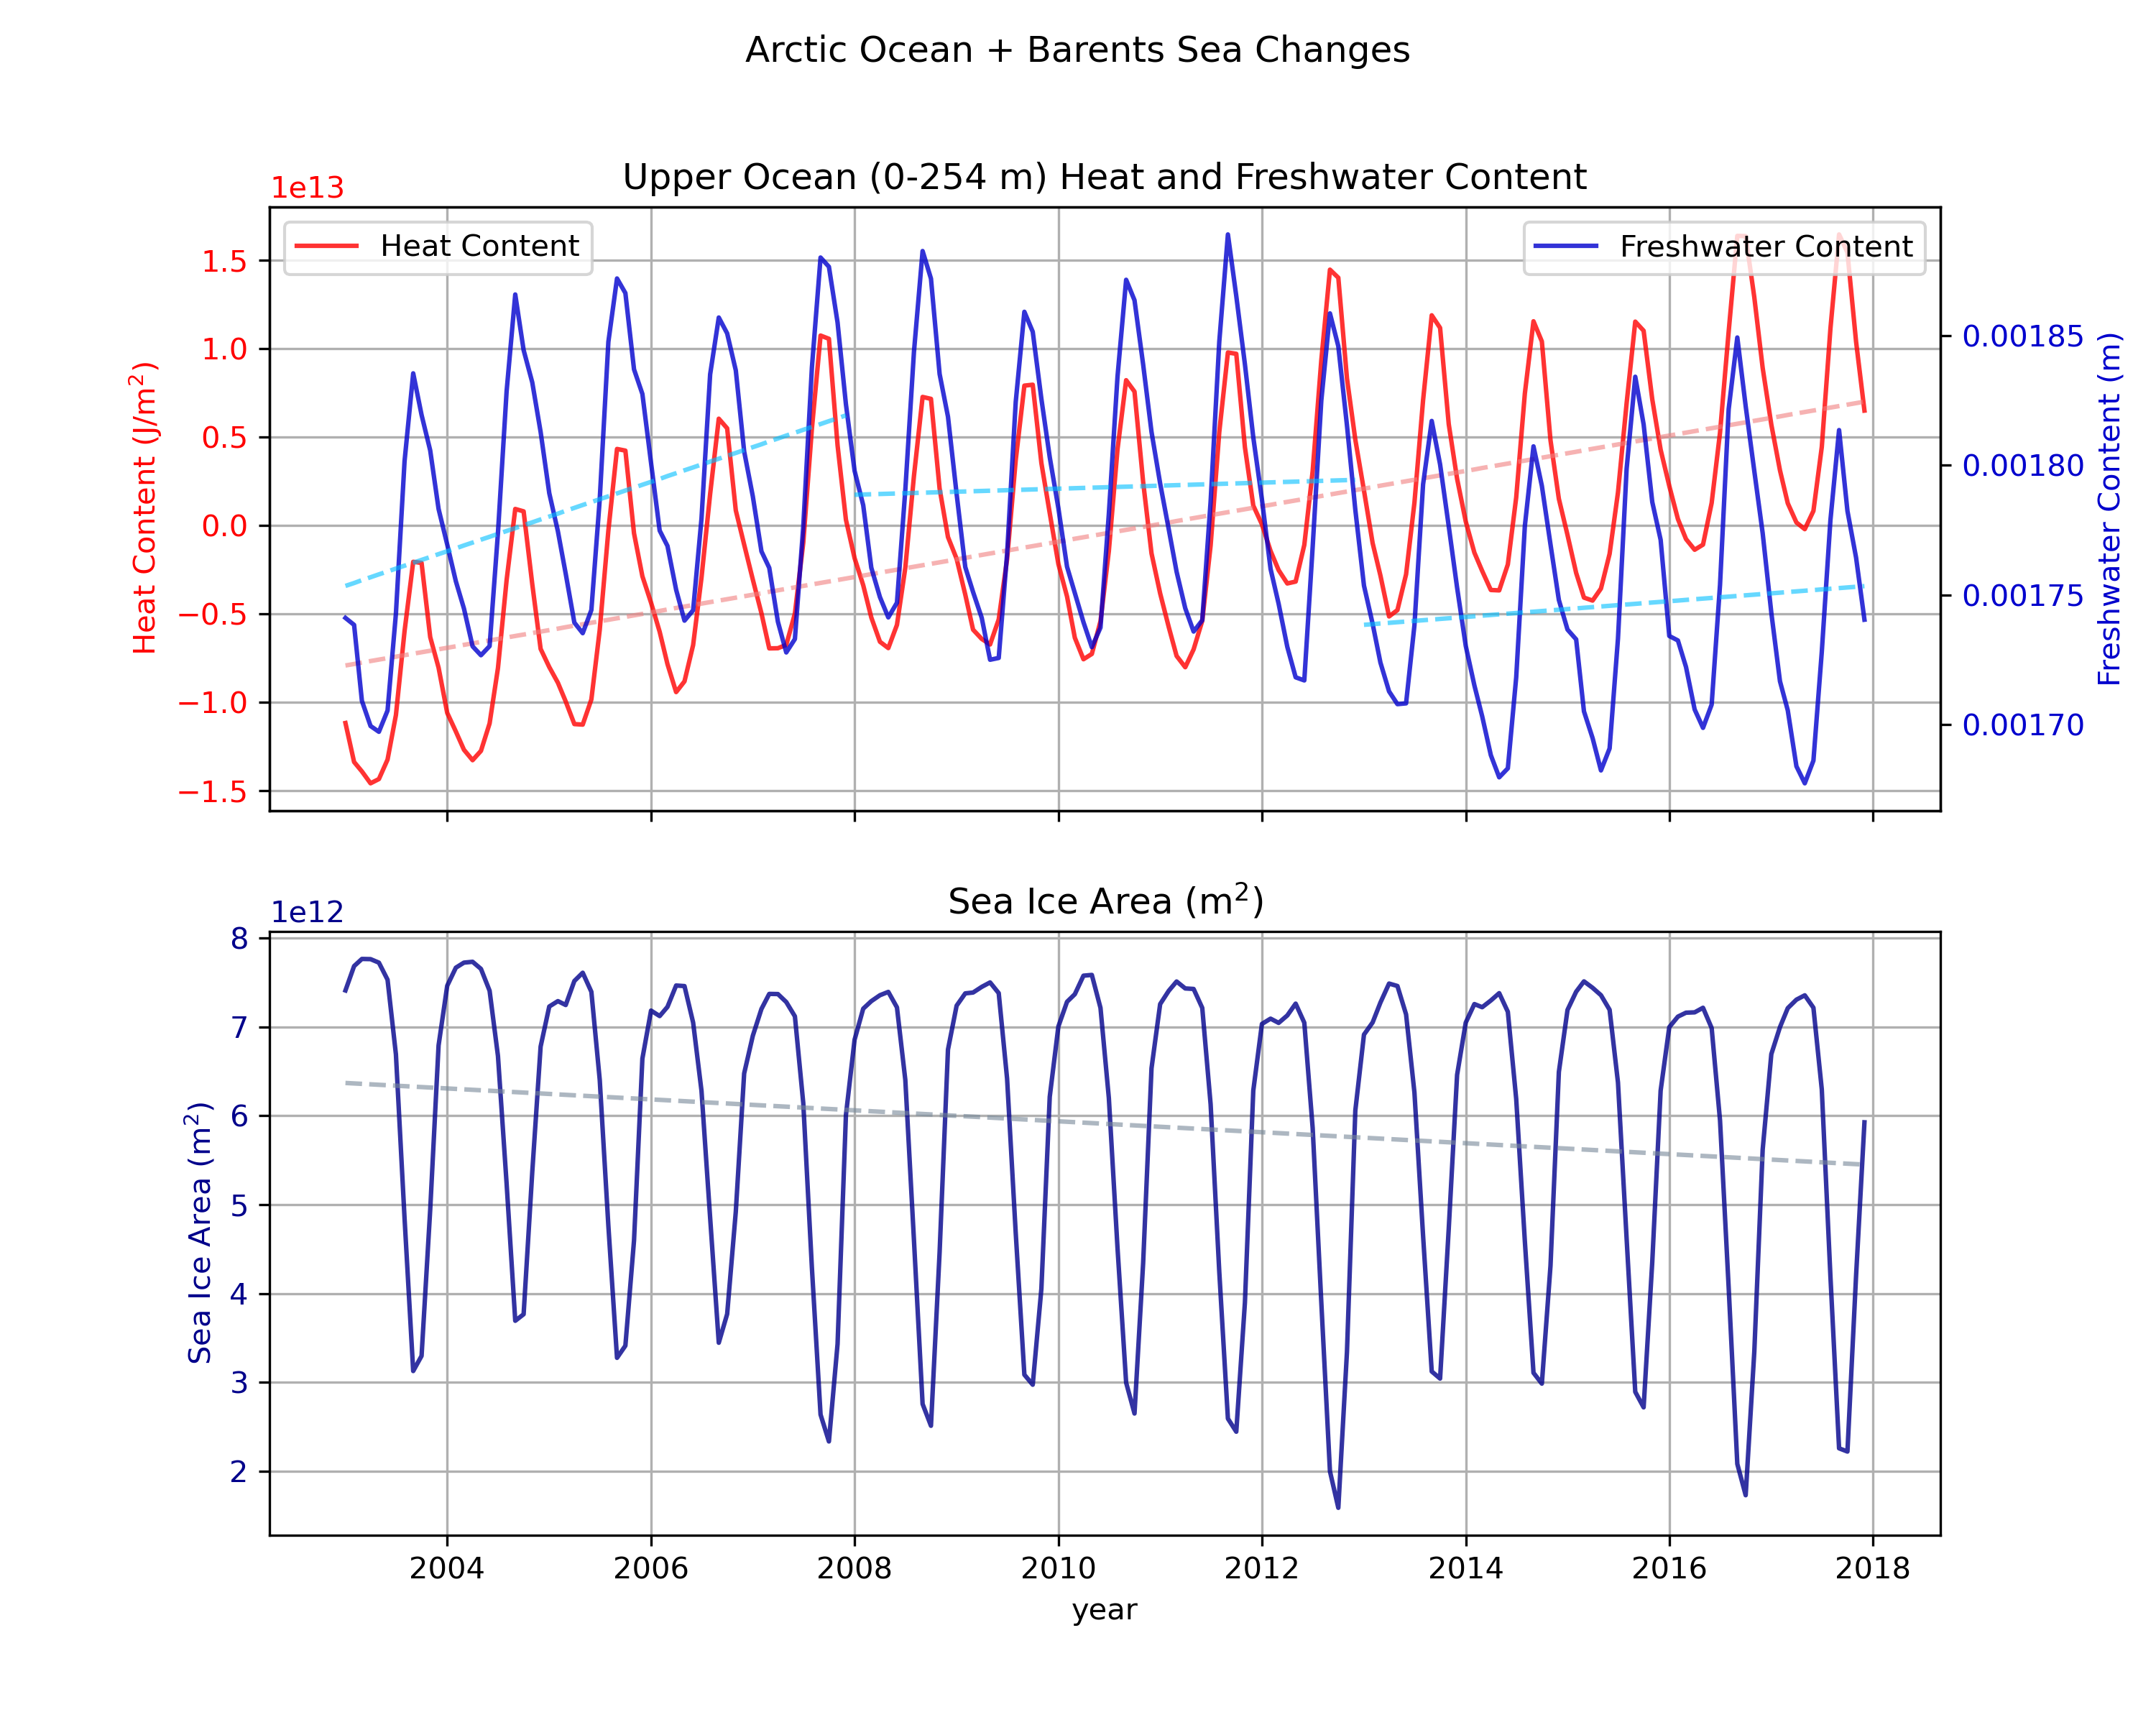
\includegraphics[width=\linewidth]{figs/Arctic_timeseries_proposal.png}
    \caption{This is an example caption that will be changed later...}
    \label{fig:timeseries}
\end{wrapfigure}


% paragraph introducing/motivating WMT in the Barents Sea/how has this been applied in other studies
As the heat and salinity of the Barents Sea change, so too does its buoyancy. Ocean stratification is determined by buoyancy---a crucial term in the vertical momentum equation. Positive buoyancy drives upward acceleration, while negative buoyancy causes downward motion, influencing the stability of the water column. In a stratified ocean, buoyancy depends on density, which acts to restore displaced fluid particles to maintain equilibrium. In seawater, fluid density ($\rho$) depends on temperature and salt, but salinity changes exert an eight-fold greater impact on $\rho$. This makes salinity an important factor shaping stratification, particularly in polar regions where surface salt fluxes are substantial.

% role of Advection and sea ice dynamics on WMT; explain advection, transport of heat and salt through advective transport, how AW drives transformation during this process; how do sea ice dynamics affect vertical mixing and alter mixing and water mass properties
Temperature (\emph{T}) and salinity (\emph{S}) are important tracers for identifying water masses and understanding their transformation through the ocean. Water Mass Transformation (WMT) was initially studied through the analysis of flow across isohaline \cite{Walin_1977} and isothermal \cite{Walin1982} surfaces. Building on these foundational papers, a thermohaline streamfunction has been introducted (Doos, Zika 2012) and volume transport has been formulated in \emph{T}--\emph{S} space \cite{Hieronymus2014}. The WMT framework has been applied in several regions of the global ocean, including the North Atlantic \cite{Speer1993}, Arctic gateways \cite{Rudels2008}, and the Arctic Ocean basin \cite{Pemberton2015}. While these studies identified the primary drivers of buoyancy change, a limitation in WMT analysis has been the absence of fully-closed budgets. This has resulted in substantial residuals that can introduce errors into the heat and salt budgets \cite{Pemberton2015}, leaving gaps in our understanding of the relative influences of various terms in Arctic WMT.


% WMT in the Barents Sea -- what's the point
We employ a fully-closed WMT framework in \emph{T}--\emph{S} space for the Barents Sea. Closed budgets, derived from continuity equations, are essential for accurately capturing heat and freshwater variability by accounting for all contributing terms. The elimination of residuals thus allows us to ascertain the attribution of both dominant and minor physical processes on \emph{T} and \emph{S} changes. In the context of Atlantification in the Barents Sea, this framework is particularly valuable as it connects the changes in \emph{T} and \emph{S} to variations in density. The advection of AW is expected to play an important role in the observed warming and salinification of the Barents Sea, particularly in the northern, salinity-stratified regime. Surface heat fluxes and sea ice retreat further modulate surface transformation, reinforcing changes in the water column. Internal mixing contributes to WMT, homogenizing the previous contributions from advection and surface processes. Ultimately, the closed-budget WMT framework provides a comprehensive and nuanced understanding of the processes driving regime shifts in the Barents Sea, shedding light on the interplay between these processes.


% motivation and research questions; key gaps in knowledge; goals of the paper as quantifying WMT, identifying key drivers, and understanding their implications on the Arctic system
(DRAFT) We hypothesize that the relative roles of AW import and surface process changes can be quantified using a budgeted WMT framework.


\section{Methodology}\label{methods}

\subsection{Model Description}

\subsection{Budget Analysis}

% why is our budget analysis unique

% what is budget analysis

% INCLUDE the equations for this

% FIGURE 3: demonstrate budget analysis in T--S space

\subsection{Temperature--Salinity Analysis}

% FIGURE 4: for the 5 years; motivate this with figure 1 (SI extent timeseries)
% goal of this is to show that the advective term is changing over time as a contribution to heating and salting

\section{Results}

% FIGURE 5: highlight the convergence anomalies for the five years; compare this to figure 2 with the vertical stratification (redistribution away from the center to make a more average looking profile)
% focus on the one month (march) or maybe take a winter average motivated by the literature, use this for 2012 and 2014 to show that less sea ice -- less stratification -- redistribution of water away from the mixing line


%%

%  Numbered lines in equations:
%  To add line numbers to lines in equations,
%  \begin{linenomath*}
%  \begin{equation}
%  \end{equation}
%  \end{linenomath*}



%% Enter Figures and Tables near as possible to where they are first mentioned:
%
% DO NOT USE \psfrag or \subfigure commands.
%
% Figure captions go below the figure.
% Acronyms used in figure captions will be spelled out in the final, published version.

% Table titles go above tables;  other caption information
%  should be placed in last line of the table, using
% \multicolumn2l{$^a$ This is a table note.}
% NOTE that there is no difference between table caption and table heading in the final, published version
%
%----------------
% EXAMPLE FIGURES
%
% \begin{figure}
% \includegraphics{example.png}
% \caption{caption}
% \end{figure}
%
% Giving latex a width will help it to scale the figure properly. A simple trick is to use \textwidth. Try this if large figures run off the side of the page.
% \begin{figure}
% \noindent\includegraphics[width=\textwidth]{anothersample.png}
%\caption{caption}
%\label{pngfiguresample}
%\end{figure}
%
%
% If you get an error about an unknown bounding box, try specifying the width and height of the figure with the natwidth and natheight options. This is common when trying to add a PDF figure without pdflatex.
% \begin{figure}
% \noindent\includegraphics[natwidth=800px,natheight=600px]{samplefigure.pdf}
%\caption{caption}
%\label{pdffiguresample}
%\end{figure}
%
%
% PDFLatex does not seem to be able to process EPS figures. You may want to try the epstopdf package.
%

%
% ---------------
% EXAMPLE TABLE
%
% \begin{table}
% \caption{Time of the Transition Between Phase 1 and Phase 2$^{a}$}
% \centering
% \begin{tabular}{l c}
% \hline
%  Run  & Time (min)  \\
% \hline
%   $l1$  & 260   \\
%   $l2$  & 300   \\
%   $l3$  & 340   \\
%   $h1$  & 270   \\
%   $h2$  & 250   \\
%   $h3$  & 380   \\
%   $r1$  & 370   \\
%   $r2$  & 390   \\
% \hline
% \multicolumn{2}{l}{$^{a}$Footnote text here.}
% \end{tabular}
% \end{table}

%%%%%%%%%%%%%%%%%%%%%%%%%%%%%%%%%%%%%%%%%%%%%%%
% SIDEWAYS FIGURES and TABLES
% AGU prefers the use of {sidewaystable} over {landscapetable} as it causes fewer problems.
%
% \begin{sidewaysfigure}
% \includegraphics[width=20pc]{figsamp}
% \caption{caption here}
% \label{newfig}
% \end{sidewaysfigure}
%
%  \begin{sidewaystable}
%  \caption{Caption here}
% \label{tab:signif_gap_clos}
%  \begin{tabular}{ccc}
% one&two&three\\
% four&five&six
%  \end{tabular}
%  \end{sidewaystable}

%% If using numbered lines, please surround equations with \begin{linenomath*}...\end{linenomath*}
%\begin{linenomath*}
%\begin{equation}
%y|{f} \sim g(m, \sigma),
%\end{equation}
%\end{linenomath*}

%%% End of body of article

%%%%%%%%%%%%%%%%%%%%%%%%%%%%%%%%%%%%%%%%%%%%%%%
%% Optional Appendices go here
%
% The \appendix command resets counters and redefines section heads
%
% After typing \appendix
%
%\section{Here Is Appendix Title}
% will show
% A: Here Is Appendix Title
%
%\appendix
%\section{Here is a sample appendix}

%%%%%%%%%%%%%%%%%%%%%%%%%%%%%%%%%%%%%%%%%%%%%%%
% Optional Glossary, Notation or Acronym section goes here:
%
% Glossary is only allowed in Reviews of Geophysics
%  \begin{glossary}
%  \term{Term}
%   Term Definition here
%  \term{Term}
%   Term Definition here
%  \term{Term}
%   Term Definition here
%  \end{glossary}


%%%%%%%%%%%%%%%%%%%%%%%%%%%%%%%%%%%%%%%%%%%%%%%
% Acronyms
%% NOTE that acronyms in the final published version will be spelled out when used in figure captions.
%   \begin{acronyms}
%   \acro{Acronym}
%   Definition here
%   \acro{EMOS}
%   Ensemble model output statistics
%   \acro{ECMWF}
%   Centre for Medium-Range Weather Forecasts
%   \end{acronyms}


%%%%%%%%%%%%%%%%%%%%%%%%%%%%%%%%%%%%%%%%%%%%%%%
% Notation
%   \begin{notation}
%   \notation{$a+b$} Notation Definition here
%   \notation{$e=mc^2$}
%   Equation in German-born physicist Albert Einstein's theory of special
%  relativity that showed that the increased relativistic mass ($m$) of a
%  body comes from the energy of motion of the body—that is, its kinetic
%  energy ($E$)—divided by the speed of light squared ($c^2$).
%   \end{notation}




%%%%%%%%%%%%%%%%%%%%%%%%%%%%%%%%%%%%%%%%%%%%%%%
%
% DATA SECTION and ACKNOWLEDGMENTS
%
%%%%%%%%%%%%%%%%%%%%%%%%%%%%%%%%%%%%%%%%%%%%%%%

\section*{Open Research Section}
The ASTE\_R1 model configuration, inputs, and monthly and daily outputs are available at the Arctic Data Center (https://arcticdata.io).


\acknowledgments
Enter acknowledgments here. This section is to acknowledge funding, thank colleagues, enter any secondary affiliations, and so on.


%%%%%%%%%%%%%%%%%%%%%%%%%%%%%%%%%%%%%%%%%%%%%%%
% REFERENCES and BIBLIOGRAPHY
%
\bibliography{agusample} %don't specify the file extension
% don't specify bibliographystyle
%
%%%%%%%%%%%%%%%%%%%%%%%%%%%%%%%%%%%%%%%%%%%%%%%

%\bibliography{ enter your bibtex bibliography filename here }



%Reference citation instructions and examples:
%
% Please use ONLY \cite and \citeA for reference citations.
% \cite for parenthetical references
% ...as shown in recent studies (Simpson et al., 2019)
% \citeA for in-text citations
% ...Simpson et al. (2019) have shown...
%
%
%...as shown by \citeA{jskilby}.
%...as shown by \citeA{lewin76}, \citeA{carson86}, \citeA{bartoldy02}, and \citeA{rinaldi03}.
%...has been shown \cite{jskilbye}.
%...has been shown \cite{lewin76,carson86,bartoldy02,rinaldi03}.
%... \cite <i.e.>[]{lewin76,carson86,bartoldy02,rinaldi03}.
%...has been shown by \cite <e.g.,>[and others]{lewin76}.
%
% apacite uses < > for prenotes and [ ] for postnotes
% DO NOT use other cite commands (e.g., \citet, \citep, \citeyear, \nocite, \citealp, etc.).
%



\end{document}



More Information and Advice:

%%%%%%%%%%%%%%%%%%%%%%%%%%%%%%%%%%%%%%%%%%%%%%%
%
%  SECTION HEADS
%
%%%%%%%%%%%%%%%%%%%%%%%%%%%%%%%%%%%%%%%%%%%%%%%

% Capitalize the first letter of each word (except for
% prepositions, conjunctions, and articles that are
% three or fewer letters).

% AGU follows standard outline style; therefore, there cannot be a section 1 without
% a section 2, or a section 2.3.1 without a section 2.3.2.
% Please make sure your section numbers are balanced.
% ---------------
% Level 1 head
%
% Use the \section{} command to identify level 1 heads;
% type the appropriate head wording between the curly
% brackets, as shown below.
%
%An example:
%\section{Level 1 Head: Introduction}
%
% ---------------
% Level 2 head
%
% Use the \subsection{} command to identify level 2 heads.
%An example:
%\subsection{Level 2 Head}
%
% ---------------
% Level 3 head
%
% Use the \subsubsection{} command to identify level 3 heads
%An example:
%\subsubsection{Level 3 Head}
%
%---------------
% Level 4 head
%
% Use the \subsubsubsection{} command to identify level 3 heads
% An example:
%\subsubsubsection{Level 4 Head} An example.
%
%%%%%%%%%%%%%%%%%%%%%%%%%%%%%%%%%%%%%%%%%%%%%%%
%
%  IN-TEXT LISTS
%
%%%%%%%%%%%%%%%%%%%%%%%%%%%%%%%%%%%%%%%%%%%%%%%
%
% Do not use bulleted lists; enumerated lists are okay.
% \begin{enumerate}
% \item
% \item
% \item
% \end{enumerate}
%
%%%%%%%%%%%%%%%%%%%%%%%%%%%%%%%%%%%%%%%%%%%%%%%
%
%  EQUATIONS
%
%%%%%%%%%%%%%%%%%%%%%%%%%%%%%%%%%%%%%%%%%%%%%%%

% Single-line equations are centered.
% Equation arrays will appear left-aligned.

Math coded inside display math mode \[ ...\]
 will not be numbered, e.g.,:
 \[ x^2=y^2 + z^2\]

 Math coded inside \begin{equation} and \end{equation} will
 be automatically numbered, e.g.,:
 \begin{equation}
 x^2=y^2 + z^2
 \end{equation}


% To create multiline equations, use the
% \begin{eqnarray} and \end{eqnarray} environment
% as demonstrated below.
\begin{eqnarray}
  x_{1} & = & (x - x_{0}) \cos \Theta \nonumber \\
        && + (y - y_{0}) \sin \Theta  \nonumber \\
  y_{1} & = & -(x - x_{0}) \sin \Theta \nonumber \\
        && + (y - y_{0}) \cos \Theta.
\end{eqnarray}

%If you don't want an equation number, use the star form:
%\begin{eqnarray*}...\end{eqnarray*}

% Break each line at a sign of operation
% (+, -, etc.) if possible, with the sign of operation
% on the new line.

% Indent second and subsequent lines to align with
% the first character following the equal sign on the
% first line.

% Use an \hspace{} command to insert horizontal space
% into your equation if necessary. Place an appropriate
% unit of measure between the curly braces, e.g.
% \hspace{1in}; you may have to experiment to achieve
% the correct amount of space.


%%%%%%%%%%%%%%%%%%%%%%%%%%%%%%%%%%%%%%%%%%%%%%%
%
%  EQUATION NUMBERING: COUNTER
%
%%%%%%%%%%%%%%%%%%%%%%%%%%%%%%%%%%%%%%%%%%%%%%%

% You may change equation numbering by resetting
% the equation counter or by explicitly numbering
% an equation.

% To explicitly number an equation, type \eqnum{}
% (with the desired number between the brackets)
% after the \begin{equation} or \begin{eqnarray}
% command.  The \eqnum{} command will affect only
% the equation it appears with; LaTeX will number
% any equations appearing later in the manuscript
% according to the equation counter.
%

% If you have a multiline equation that needs only
% one equation number, use a \nonumber command in
% front of the double backslashes (\\) as shown in
% the multiline equation above.

% If you are using line numbers, remember to surround
% equations with \begin{linenomath*}...\end{linenomath*}

%  To add line numbers to lines in equations:
%  \begin{linenomath*}
%  \begin{equation}
%  \end{equation}
%  \end{linenomath*}



